\subsection{Layout dell'apparato e Frame}

Per la realizzazione dell’esperimento è necessario realizzare una struttura di supporto in cui poter fissare i differenti rivelatori. Le linee guida per il progetto sono state essenzialmente tre: 1) Leggerezza della struttura; 2) Resistenza termica; 3) Facilità di realizzazione. Per soddisfare questi tre punti si è deciso di realizzare una struttura stampata in 3D; il materiale che più si adatta alle richieste è il PETG, un materiale meccanicamente e termicamente resistente e che inoltre è facilmente stampabile. 
Da esperimenti eseguiti su questo materiale si è visto che con un trattamento termico (“thermal annealing”) in cui si raggiungono i -40°C, il materiale perde solamente il 2-3\% delle caratteristiche meccaniche. Per quanto riguarda la temperatura massima, la temperatura di transizione vetrosa del materiale è 80°C, oltre la quale il materiale passa a perdere le proprie caratteristiche di rigidezza ed assume un comportamento gommoso. Dai dati di precedenti voli si è visto che le temperature più alte vengono raggiunte solamente localmente dai compenti elettronici, pertanto anche se si dovessero superare i 70°C non sarebbe un problema per la resistenza strutturale dei supporti. 
In Figura \ref{frame} è riportato il supporto meccanico assemblato con i rivelatori.
\begin{figure}
    \centering
    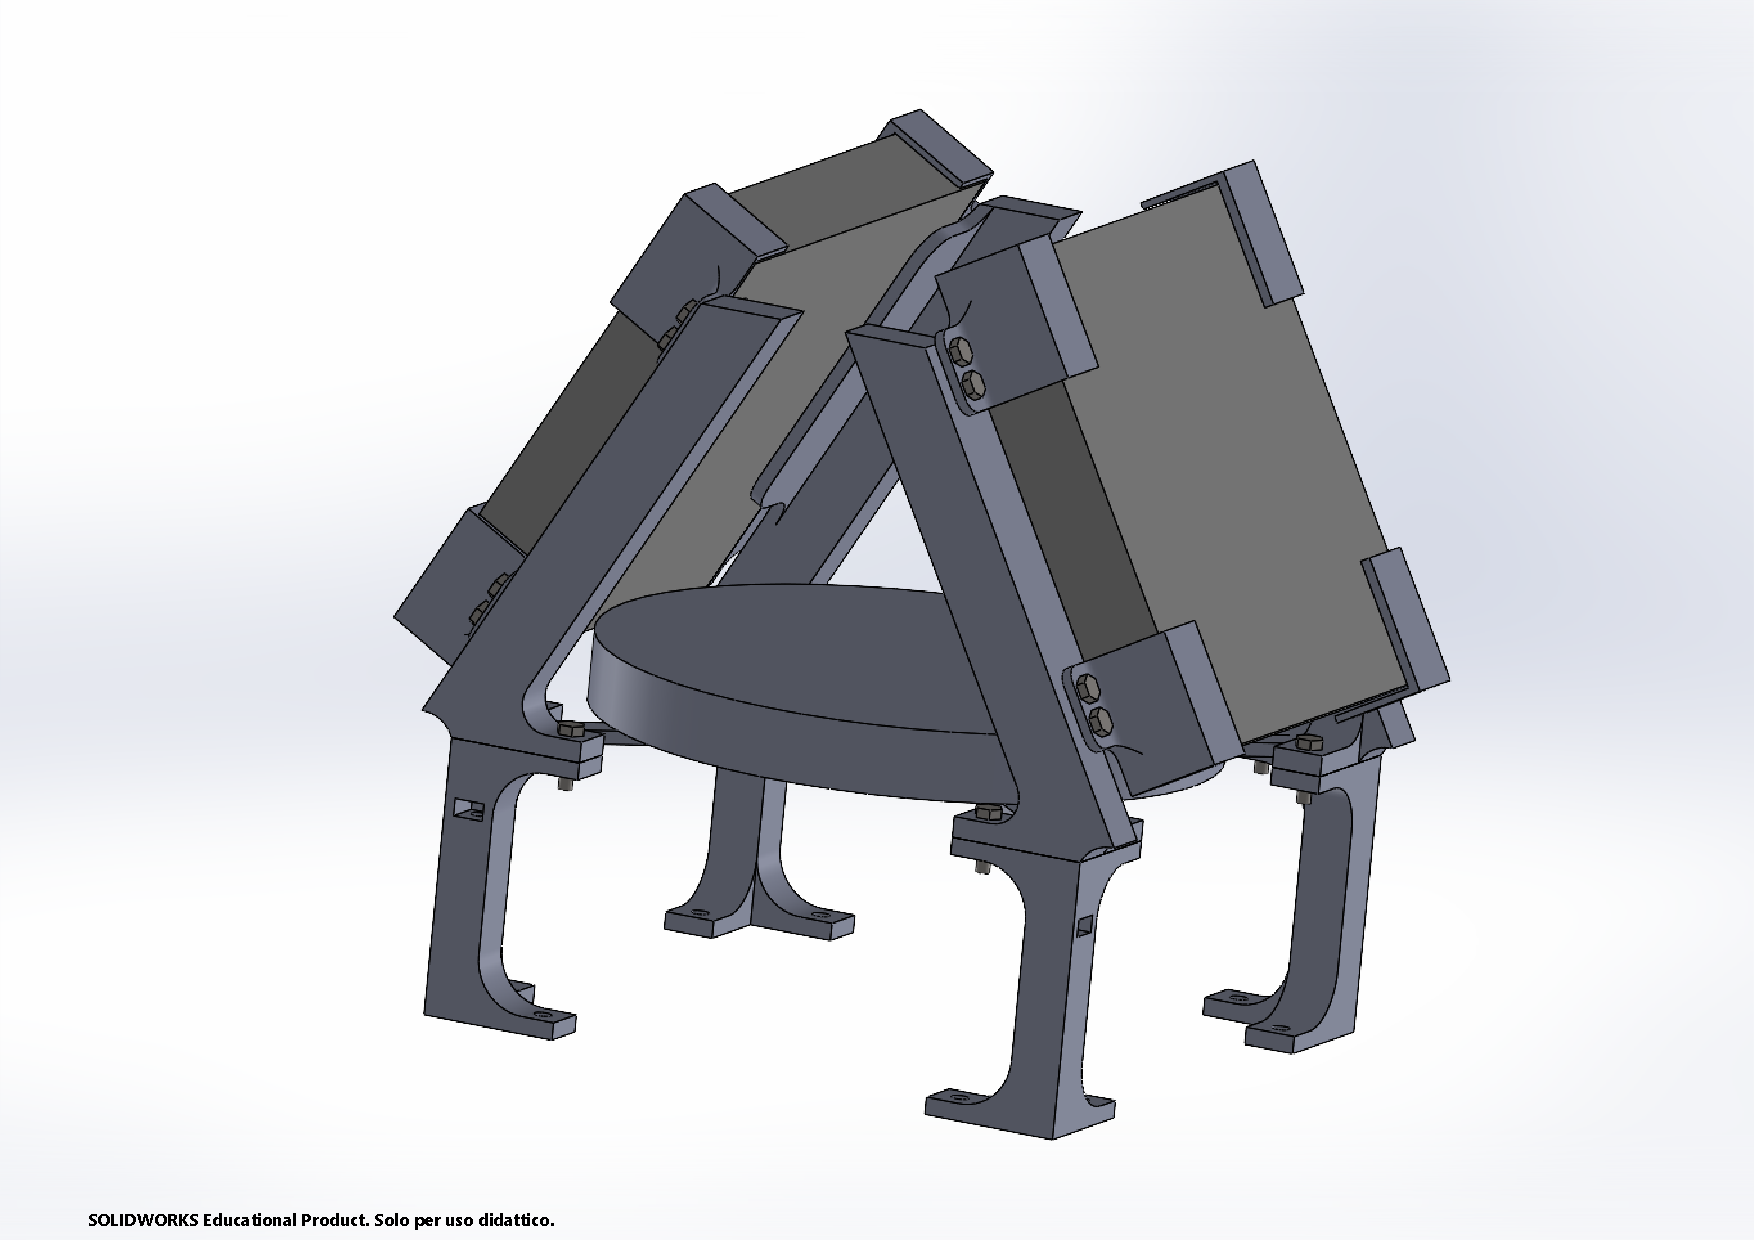
\includegraphics[width=0.4\textwidth]{definitivo___FORSE2.2.PDF}
    \\
    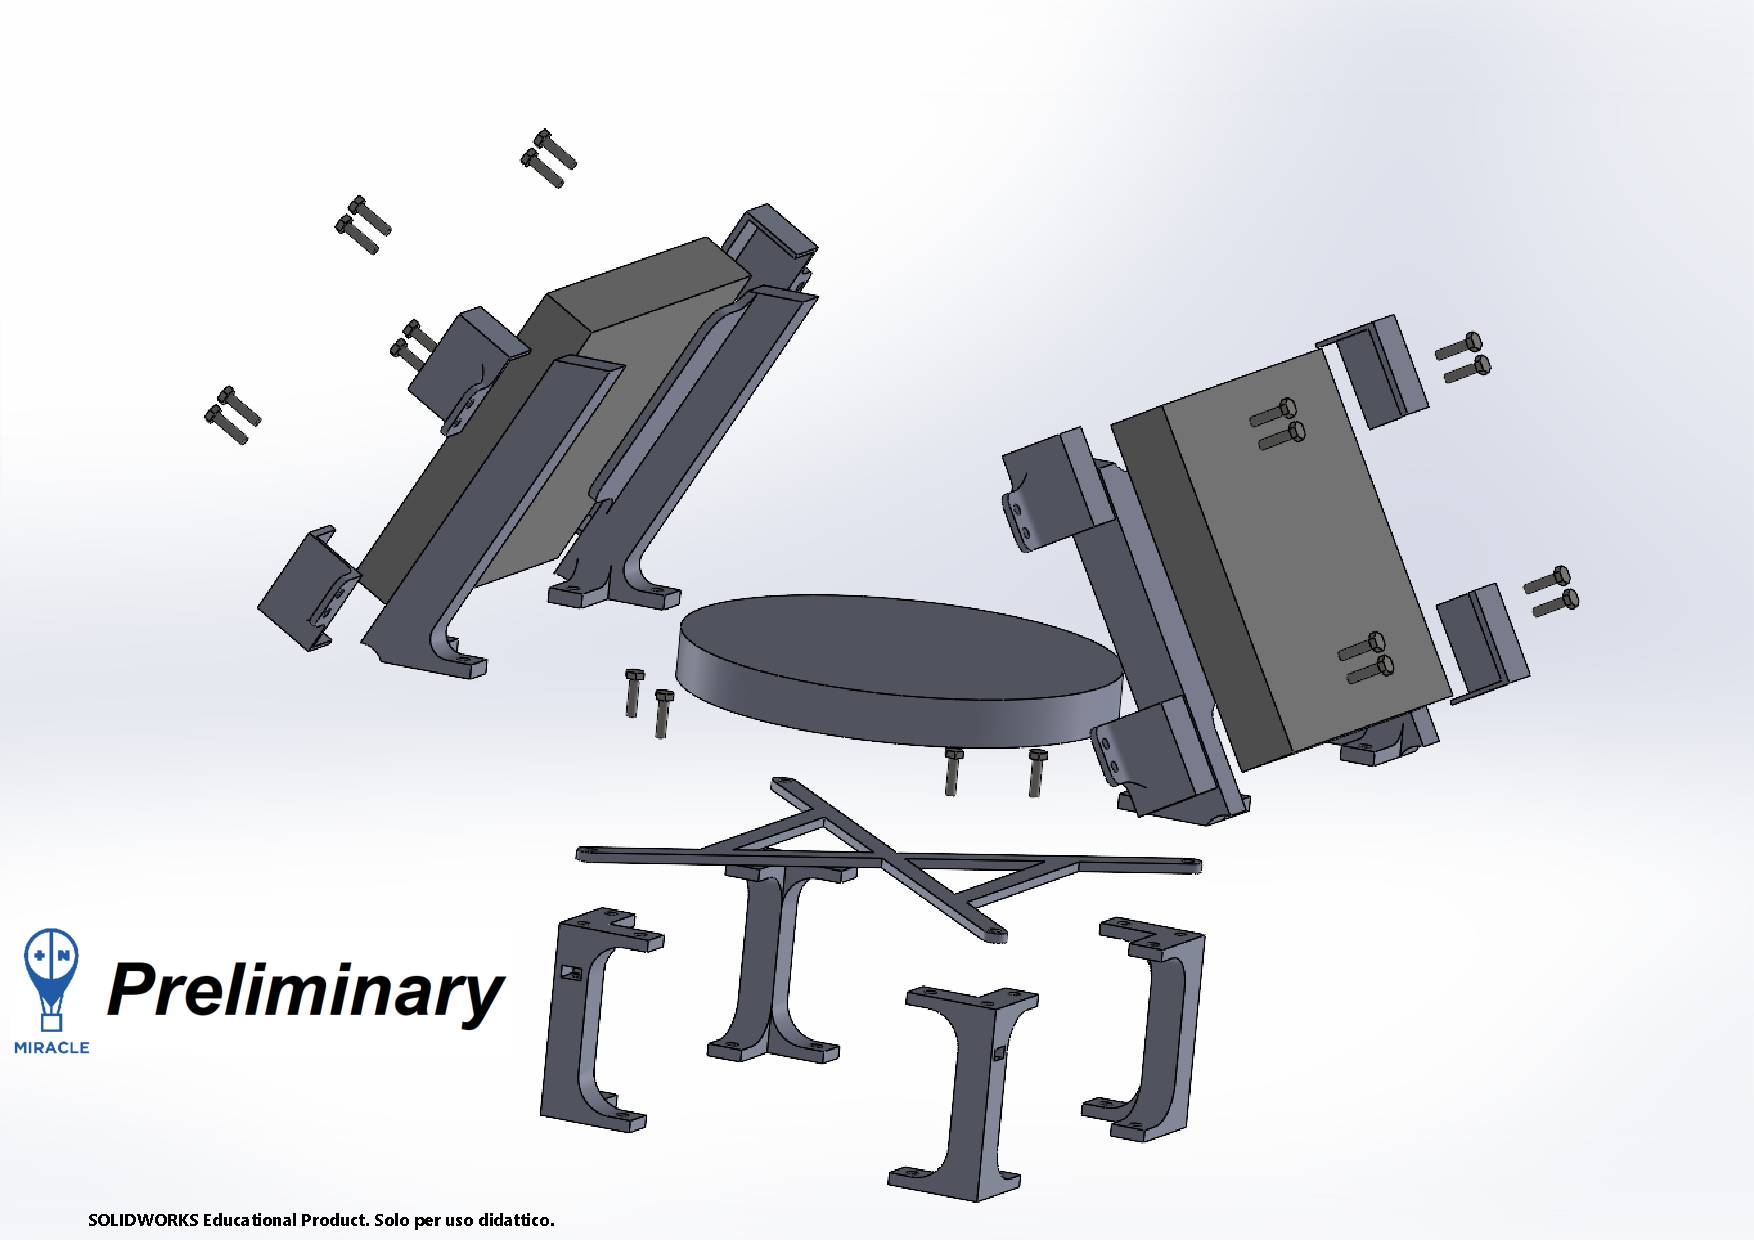
\includegraphics[width=0.4\textwidth]{ESPLOSO2.2.PDF}

    \caption{Sopra: frame di sostegno con rivelatori montati; sotto: vista esplosa. In obliquo vengono allocati gli scintillatori, mentre al centro viene posizionata la micromegas; sottostante la micromegas, viene posizionato il rivelatore di neutroni.}
    \label{frame}
\end{figure}
Si è deciso di utilizzare una configurazione a \emph{tetto} per minimizzare peso e spazio occupato, senza rinunciare a misure di flusso orizzontale (coincidenza tra i due scintillatori) e verticale (scintillatori in anticoincidenza tra loro + scintillatori in coincidenza con la micromegas).
In questa configurazione, il rivelatore di neutroni viene alloggiato sotto la micromegas.